
% \vspace{-10mm}
\section{Experiments}
\label{sec:exp}

We report on extensive experiments aimed at evaluating the performance of  \ClusterEA{}.

\begin{table}[t]\small
\centering
\caption{Statistics of IDS15K, IDS100K and DBP1M.}
\vspace{-4mm}
\label{tb:dataset}
\setlength{\tabcolsep}{0.4mm}{
\begin{tabular}{ll|l|l|l}
\toprule
\multicolumn{2}{c|}{Datasets}                          & \#Entities          & \#Relations & \#Triples           \\ \hline
\multicolumn{1}{l|}{\multirow{2}{*}{IDS15K}}  & EN-FR & 15,000-15,000       & 267-210     & 47,334-40,864       \\
\multicolumn{1}{l|}{}                         & EN-DE & 15,000-15,000       & 215-131     & 47,676-50,419       \\ \hline
\multicolumn{1}{l|}{\multirow{2}{*}{IDS100K}} & EN-FR & 100,000-100,000     & 400-300     & 309,607-258,285     \\
\multicolumn{1}{l|}{}                         & EN-DE & 100,000-100,000     & 381-196     & 335,359-336,240     \\ \hline
\multicolumn{1}{l|}{\multirow{2}{*}{DBP1M}}   & EN-FR & 1,877,793-1,365,118 & 603-380     & 7,031,172-2,997,457 \\
\multicolumn{1}{l|}{}                         & EN-DE & 1,625,999-1,112,970 & 597-241     & 6,213,639-1,994,876 \\ \bottomrule
\end{tabular}}
\end{table}  

\vspace{-2mm}
\subsection{Experimental Settings}\label{sec:exp_setting}


\begin{table*}[t]\small
% \vspace*{-22mm}
\caption{Overall EA results on IDS15K and IDS100K
}\label{exp:overall_15K_100K}
\vspace*{-4mm}
\begin{threeparttable}
\setlength{\tabcolsep}{0.6mm}{
\begin{tabular}{l|ccccc|ccccc|ccccc|ccccc}
\toprule
\multicolumn{1}{c|}{\multirow{2}{*}{Methods}} & \multicolumn{5}{c|}{IDS15K$_{EN-FR}$} & \multicolumn{5}{c|}{IDS15K$_{EN-DE}$} & \multicolumn{5}{c|}{IDS100K$_{EN-FR}$} & \multicolumn{5}{c}{IDS100K$_{EN-DE}$} \\ \cline{2-21}
 &  H@1 &  H@10 & MRR & Time &  Mem. & H@1 &  H@10 & MRR & Time &  Mem. &  H@1 &  H@10 & MRR & Time  &  Mem. &  H@1 &  H@10 & MRR & Time  &  Mem.\\ \hline
GCNAlign   & 38.2 & 78.5 & 0.51 & 10.90 &\textbf{ 0.13} & 58.7 & 85.5 & 0.67 & 12.27 &\textbf{ 0.13} & 29.9 & 61.7 & 0.40 & 71.37 & 1.00 & 41.0 & 66.1 & 0.49 & 79.52 & 1.00 \\
RREA       & 63.3 & 91.4 & 0.73 & 136.32 & 4.07  & 75.5 & 94.9 & 0.82 & 156.85 & 4.07  & --    &  --   &  --   &--  & -- &      --  &   --  &  --   & --  & -- \\
Dual-AMN       & 64.6 & \textbf{91.5} & 0.74 & 12.50 & 4.05  & 76.5 & \textbf{95.2} & 0.83 & 13.72 & 4.05  & 49.3    &  77.5  &  0.59   &413.73  & 21.91 &  59.3  &  81.8  &  0.67   & 456.87  & 22.56 \\
\hline
LargeEA-G & 30.0 & 63.5 & 0.39 &\textbf{ 9.76}  & \textbf{0.13} & 40.3 & 68.7 & 0.50 & \textbf{9.94} & \textbf{0.13} & 19.5  & 45.7 & 0.28 &\textbf{ 36.65 }&  \textbf{0.50}  & 21.4 & 39.7 & 0.27 & \textbf{39.29} & \textbf{0.50} \\
LargeEA-R & 47.2 & 74.0 & 0.56 & 41.01  & 1.01 & 58.0 & 77.6 & 0.65 & 42.12  & 1.01  & 32.5 & 55.5 & 0.40 & 163.92  & 4.04 & 27.3 & 42.5 & 0.32 & 157.15 & 4.04 \\
LargeEA-D & 45.7 & 69.6 & 0.54 & 13.51  & 0.75 & 58.7 & 76.2 & 0.65 & 13.96 & 0.75 & 33.0 & 54.8 & 0.40 & 134.5  & 3.41  & 28.6 & 42.7 & 0.65 & 121.9  & 3.65  \\
GCN-Align-S & 37.1 & 73.8 & 0.49 & 24.10  & 1.11 & 53.6 & 83.4 & 0.63 & 23.73 & 1.11 & 25.3 & 45.5 & 0.35 & 184.43  & 1.72  & 35.5 & 61.5 & 0.44 & 189.12  & 1.72  \\
RREA-S & 62.7 & 90.3 & 0.72 & 34.09  & 4.89 & 76.3 & 95.0 & 0.83 & 34.23 & 5.01 & 46.4 & 75.4 & 0.56 & 250.80  & 7.16  & 57.3 & 80.6 & 0.65 & 256.35  & 8.50 \\
Dual-AMN-S & 60.9 & 88.9 & 0.71 & 15.59  & 5.30 & 75.0 & 94.3 & 0.82 & 15.64  & 5.10 & 48.2 & 76.6 & 0.57 & 122.78  & 7.79  & 58.8 & 81.4 & 0.66 & 124.49  & 8.13 \\
\textbf{\ClusterEA{-G}} & 46.6 & 77.8 & 0.57 & 40.99  & 4.43 & 62.0 & 86.3 & 0.70 & 40.47 & 4.43 & 30.6 & 57.9 & 0.40 & 236.37 & 2.77  & 41.4 & 64.3 & 0.49 & 246.90 & 2.77  \\
\textbf{\ClusterEA{-R}} & \textbf{67.9} & 90.0 & \textbf{0.76} & 52.29  & 4.89 & 79.4 & 94.5 & \textbf{0.85} & 51.89  & 5.01  & 52.0 & 76.3 & 0.60 & 329.78  & 7.16 & 62.2 & 81.7 & 0.69 & 339.54 & 8.50 \\
\textbf{\ClusterEA{-D}} & 67.4 & 89.5 & 0.75 & 35.76 & 5.30 & \textbf{79.5} & 94.6 & \textbf{0.85} & 35.82  & 5.10  & \textbf{54.2} & \textbf{78.1} & \textbf{0.62} & 210.50  & 8.52 & \textbf{63.7} & \textbf{82.8} & \textbf{0.70} & 212.80 & 8.31 \\
\bottomrule
\end{tabular}}
\begin{tablenotes}
\footnotesize
    \item[1] The symbol ``--'' indicates that the model fails to perform EA on IDS100K dataset due to extensive PU memory usage.
\end{tablenotes}
\end{threeparttable}
\vspace{-4mm}
\end{table*}


\noindent
\textbf{Datasets.}
We conduct experiments on datasets with different sizes from two cross-lingual EA benchmarks, i.e., IDS~\cite{OpenEA2020VLDB} and DBP1M~\cite{LargeEA22}. 
\begin{itemize}[topsep=0pt,itemsep=0pt,parsep=0pt,partopsep=0pt,leftmargin=*]
\item 
\emph{IDS} contains four cross-lingual datasets, i.e., English and French (IDS15K$_{EN-FR}$ and IDS100K$_{EN-FR}$), and English and German (IDS15K$_{EN-DE}$ and IDS100K$_{EN-DE}$). \MARK{These benchmarks are sampled with consideration of keeping the properties (e.g., degree distribution) consistent with their source KGs.} We use the latest 2.0 version of IDS, where the URIs of entities are encoded to avoid possible name bias.
\item \emph{DBP1M} is the largest cross-lingual benchmark for EA. It contains two large-scale cross-lingual datasets extracted from DBpedia~\cite{DBPedia}, i.e., English and French (DBP1M$_{EN-FR}$), and English and German (DBP1M$_{EN-DE}$). 
However, DBP1M is biased with name information. To be specific, part of the entities in inter-language links (ILLs) does not occur in the two KGs. We thus remove those ILLs to resolve the name bias issue while retaining all the triples.
\end{itemize}

Following previous works, we use 30\% of each dataset as seed alignment and use 70\% of it to test the EA performance.
As can be seen, we consider both degree distribution issue~\cite{RSN19, OpenEA2020VLDB} and the name bias issue~\cite{AttrGNN20} when selecting benchmarks, which meets the requirements of real-world applications.
Table \ref{tb:dataset} lists the detailed information of datasets.

\noindent
\textbf{Evaluation metric.}
We use the widely-adopted \HitNFull{} (\HitN{}), Mean Reciprocal Rank (\MRR{}) to evaluate the accuracy of \ClusterEA{}~\cite{MTransE17,IPTransE17, GCN-Align18, KECG19, RREA20, DualAMN21, EASY21}. Here, for \HitN{}, $N$=1, 10.
Higher \HitN{} and \MRR{} indicate better performance.
In addition, we use running time and maximum GPU Memory cost (\emph{Mem.}) to evaluate the scalability of \ClusterEA{}. Specifically, running time is measured in seconds, and \emph{Mem.} is measured in Gigabytes.
% following ~\cite{LargeEA22}, running time (in seconds), and the maximum GPU Memory cost (\emph{Mem.} for short, in Gigabytes) are included for evaluating the scalability of \ClusterEA{}.
% Here, the running time means the training time of every EA approach.
% We do not consider the test time. Specifically, it is common for EA methods to use the same approach for evaluating the EA results in the test set, resulting in the similar test time of different approaches. 

\noindent
\textbf{Baselines.}
\MARK{
We only compare \ClusterEA{} with structure-only methods. If a baseline contains side information components, we remove them in order to guarantee a fair comparison
~\cite{DualAMN21, EVA20, RREA20, HyperKA20, OpenEA2020VLDB, LargeEA22}.  All the baselines are enhanced with CSLS (\SparseCSLS{} for large-scale datasets) before evaluation if possible. The implementation details and parameter settings of \ClusterEA{} and all baselines are provided in Appendix~\ref{app:details}.
% We divide the compared baselines into two major categories :
% (i) \emph{Non-scalable} ones including GCNAlign, RREA, and Dual-AMN; (ii) \emph{Scalable} ones indicating other baselines mentioned above. 
Considering the scalability of models, we divide the compared baselines into two major categories, as listed below:
% We compare \ClusterEA{} with the following representative EA models.
% \begin{itemize}[topsep=0pt,itemsep=0pt,parsep=0pt,partopsep=0pt,leftmargin=*]
%     \item  \emph{GCNAlign}~\cite{GCN-Align18}: it is the first GNN based EA model. We re-implement GCNAlign by removing attribute features (as the side information component) from it.
%     \item \emph{LargeEA}~\cite{LargeEA22}: it is the first EA framework that focuses on scalability by training multiple EA models on mini-batches generated by a rule-based strategy. We reproduce LargeEA by removing the name channel entirely, including the name-based data augmentation. Excepted for the two variants introduced in~\cite{LargeEA22}, 
%     we provide a new variant \emph{LargeEA-D} that incorporates recently proposed EA model Dual-AMN.
%     \item \emph{RREA}~\cite{RREA20}: it is a GNN-based EA model that leverages relational reflection transformation to obtain relation-specific embeddings for each entity. It is used as the default of LargeEA~\cite{LargeEA22}.
%     \item \emph{Dual-AMN}~\cite{DualAMN21}: it is a SOTA EA model that encomprasses  Simplified Relational Attention Layer and Proxy Matching Attention Layer for modeling both intra-graph and cross-graph relations.
%     \item \emph{Stochastic training (Section~\ref{sec:mini-batch-training}) variant of GNN models}, that incorporates EA models with Stochastic training, including \emph{GCNAlign-S} for GCNAlign~\cite{GCN-Align18}, \emph{RREA-S} for RREA~\cite{RREA20} and \emph{Dual-AMN-S} for Dual-AMN~\cite{DualAMN21}.
% \end{itemize}
\begin{itemize}[topsep=0pt,itemsep=0pt,parsep=0pt,partopsep=0pt,leftmargin=*]
    \item \emph{Non-scalable baselines} that includes 
            (i) \emph{GCNAlign}~\cite{GCN-Align18}, the first GNN-based EA model; 
            (ii) \emph{RREA}~\cite{RREA20}, a GNN-based EA model that leverages relational reflection transformation to obtain relation-specific embeddings for each entity. It is used as the default of LargeEA~\cite{LargeEA22}; and
            (iii) \emph{Dual-AMN}~\cite{DualAMN21}, a SOTA EA model that encomprasses Simplified Relational Attention Layer and Proxy Matching Attention Layer for modeling both intra-graph and cross-graph relations.
    \item \emph{Scalable baselines} that includes 
            (i) \emph{LargeEA}~\cite{LargeEA22}, the first EA framework that focuses on scalability by training multiple EA models on mini-batches generated by a rule-based strategy. Excepted for the two variants introduced in~\cite{LargeEA22}, 
            we provide a new variant \emph{LargeEA-D} that incorporates recently proposed EA model Dual-AMN; and
            (ii) \emph{Stochastic training (Section~\ref{sec:mini-batch-training}) variant of GNN models}, that incorporates EA models with Stochastic training, including \emph{GCNAlign-S} for GCNAlign~\cite{GCN-Align18}, \emph{RREA-S} for RREA~\cite{RREA20} and \emph{Dual-AMN-S} for Dual-AMN~\cite{DualAMN21}.
\end{itemize}
}


\noindent
\textbf{Variants of \ClusterEA{}.}
Since \ClusterEA{} is designed to be integrated with GNN-based EA models, we present three versions of \ClusterEA{}, i.e.,  \ClusterEA{-G} that includes GCNAlign, \ClusterEA{-R} that incorporates RREA and  \ClusterEA{-D} that incorporates Dual-AMN. Specifically, we treat \ClusterEA{-D} as the default setting of \ClusterEA{}. 
% \MARK{Our current implementation includes three representative GNN-based EA models, including (i) GCN-Align~\cite{GCN-Align18}, the first GNN-based EA model; (ii) RREA~\cite{RREA20}, which is adopted by the first scalable EA framework LargeEA~\cite{LargeEA22}; and (iii) Dual-AMN~\cite{DualAMN21}, current state-of-the-art structure-only EA model.}

% \vspace*{-4mm}
\subsection{Overall Results}


\begin{table}[t]\small
\caption{Overall EA results on DBP1M}\label{exp:overall_1M}
\vspace{-4mm}
\setlength{\tabcolsep}{0.1mm}{
\begin{tabular}{l|ccccc|ccccc}
\toprule
\multicolumn{1}{c|}{\multirow{2}{*}{Methods}} & \multicolumn{5}{c|}{DBP1M$_{EN-FR}$}  & \multicolumn{5}{c}{DBP1M$_{EN-DE}$}  \\ \cline{2-11}
\multicolumn{1}{c|}{} & \multicolumn{1}{c}{H@1} & \multicolumn{1}{c}{H@10} & \multicolumn{1}{c}{MRR} & \multicolumn{1}{c}{Time} &  \multicolumn{1}{c|}{Mem.} & \multicolumn{1}{c}{H@1} & \multicolumn{1}{c}{H@10} & \multicolumn{1}{c}{MRR} & \multicolumn{1}{c}{Time} & Mem. \\ \hline
LargeEA-G & 5.1 & 13.4 & 0.08 & \textbf{463}  & \textbf{4.00G}   & 3.4 & 9.5 & 0.05 & \textbf{378} & \textbf{4.00G}\\
LargeEA-R & 9.4 & 21.5 & 0.13 & 1681  & 20.05G  & 6.4 & 15.0 & 0.09 & 1309 & 20.49G \\
LargeEA-D & 10.5 & 21.9 & 0.15 & 2546  & 19.72G  & 6.6 & 14.7 & 0.09 & 1692 & 17.71G \\
GCN-Align-S & 6.0 & 19.1  & 0.10 & 1817  & 9.25G & 4.5 & 14.4  & 0.08 & 1491  & 7.78G \\
RREA-S & 21.1 & 42.2  & 0.28 & 2080  & 16.86G  & 20.5 & 40.2  & 0.27 & 1754  & 15.65G \\
Dual-AMN-S & 22.4 & 43.4  & 0.29 & 588  & 15.85G  & 22.0 & 41.7  & 0.28 & 490  & 14.61G\\
\textbf{\ClusterEA{-G}} & 10.0 & 24.5 & 0.15 & 2501  & 17.43G  & 6.9 & 17.7 & 0.11 & 2027  & 17.76G \\
\textbf{\ClusterEA{-R}}& 26.0 & 45.6  & 0.32 & 3025  & 21.11G& 25.0 & 45.0  & 0.32 & 2526  & 19.68G \\
\textbf{\ClusterEA{-D}}& \textbf{28.1} & \textbf{47.4}  & \textbf{0.35} & 1647  & 20.10G  & \textbf{28.8} & \textbf{48.8}  & \textbf{0.35} & 1360 & 18.20G \\
\bottomrule
\end{tabular}}
\vspace*{-4.0mm}
\end{table}


\noindent
\textbf{Performance on IDS.}\label{sec:exp_ids}
Table~\ref{exp:overall_15K_100K} summarizes the EA performance on IDS15K and IDS100K.
% \noindent
% \textbf{Accuracy Evaluations.}
% We first focus on the \textbf{accuracy} for all the variants of \ClusterEA{} and its competitors.
First,  \ClusterEA{} improves \HitOne{} by   $3.3\%-29.7\%$ compared with the non-scalable methods (GCNAlign, RREA, Dual-AMN), and improves it by $3.2\%-42.3\%$ compared with the scalable ones. These validate the accuracy of \ClusterEA{}.
% 3.3 29.7 4.7 37.9
% 4.0 20.8 3.2 39.2
% 4.9 24.3 6.0 34.7
% 4.4 22.7 4.9 42.3 
% 
Moreover, all variants of \ClusterEA{} perform better than the structure-only models in terms of \HitOne{}. It validates the superiority of the way how we enhance the output compared with CSLS, which is the default setting for most recent EA models~\cite{EVA20,EASY21, MRAEA20,RREA20, OpenEA2020VLDB, DualAMN21} to enhance the output similarity matrix. 

Second, it can be seen that the accuracy of LargeEA variants is significantly reduced compared with their corresponding original models. This is because LargeEA discards structure information during its mini-batch training process. Unlike the LargeEA variants, the accuracy of Stochastic Training variants only drops slightly compared with the original non-scalable models. This verifies that the Stochastic training process can minimize the structure information loss (cf. Section~\ref{sec:mini-batch-training}). 

Third, as observed,  \HitTen{} of some non-scalable models (RREA, Dual-AMN) is higher than that of \ClusterEA{}. This is mainly because: (i) the information loss during \ClusterEA{}'s Stochastic training; and (ii) the incompleteness of global similarity normalization (to be detailed in Section~\ref{sec:ablation}). Nevertheless, \HitOne{} is the most representative indicator for evaluating the accuracy of EA since higher \HitOne{} directly indicates more correct proportion of aligned entities. Thus, achieving the highest \HitOne{} among all baselines is sufficiently to confirm the high performance of \ClusterEA{}.
%considering that \HitOne{} represents the correct proportion of aligned entities, it is the most representative indicator for evaluating the accuracy. It would be an acceptable trade-off for better \HitOne{}.

Finally, the experimental results show that the training of all LargeEA variants is faster than that of other variants of the corresponding models. This is because LargeEA omits most information of graph structure, where less data is subjected to the training process. However, in this case, the running time of \ClusterEA{} is still comparable with LargeEA.


\noindent
\textbf{Performance on DBP1M.}
Table~\ref{exp:overall_1M} reports the EA performance of \ClusterEA{} and its competitors on DBP1M. Note that we do not report the results of the non-scalable models because it is infeasible to perform their training phases on DBP1M due to extensive GPU memory usage.
We observe that the accuracy of all the variants of \ClusterEA{} on DBP1M  is higher than those of LargeEA. Specifically, \HitOne{} is improved by $5.7\%-23.0\%$ and $6.8\%-25.4\%$ on DBP1M$_{EN-FR}$ and DBP1M$_{EN-DE}$, respectively.
 
% G 4.0 2.4
% R 4.9 4.5
% D 5.7 6.8
Next, \MARK{compared with each Stochastic training variants of the corresponding incorporated model of \ClusterEA{}, \ClusterEA{} brings about $4.0\%-5.7\%$ and $2.4\%-6.8\%$ absolute improvement in \HitOne{} on DBP1M$_{EN-FR}$ and DBP1M$_{EN-DE}$ datasets, respectively. As the expressiveness of the model improves, \ClusterEA{} also provides more improvements. 
% Moreover, as observed, \ClusterEA{} is able to outperform baselines without using GNN model.
% This is because \ClusterEA{} optimizes the similarity computation via proposing a novel similarity matrix.
}
%This validates the importance of enhancing the similarity matrix and the superiority of the way of \ClusterEA{} enhancing the similarity matrix. 

% Since the Stochastic training variants are treated as a sub-module in \ClusterEA{}. 
Finally, all the scalable variants incorporating GCNAlign variants produce poor EA results. Specifically, GCNAlign's model cannot be directly applied to large-scale datasets due to its insufficient expressive ability.
\MARK{Note that \ClusterEA{} not only outperforms baselines in terms of accuracy but also achieves comparable performance with them in terms of both Mem. and running time.}
\MARK{Overall, \ClusterEA{} is able to scale-up the GNN-based EA models while enhancing \HitOne{} by at most $8\times$
%the 
%not only successfully scale-up the GNN-based EA models but also enhance the performance with up to $8\times$ improvement in terms of \HitOne{} 
compared with the state-of-the-arts. More experimental results of scalability are provided in  Appendix~\ref{app:scalability} due to the space limitation.}



\begin{figure*}[t]
\centering
\includegraphics[width=.8\textwidth]{figs/icon-1.eps}\\
\vspace*{-4mm}
\subfigure[$\rm IDS15K_{EN-FR}$]{
 \includegraphics[width=1.7in]{figs/partition-k-small-fr.eps}
 \label{fig:partition-k-small-fr}
}\hspace{-3mm}
\subfigure[$\rm IDS100K_{EN-FR}$]{
 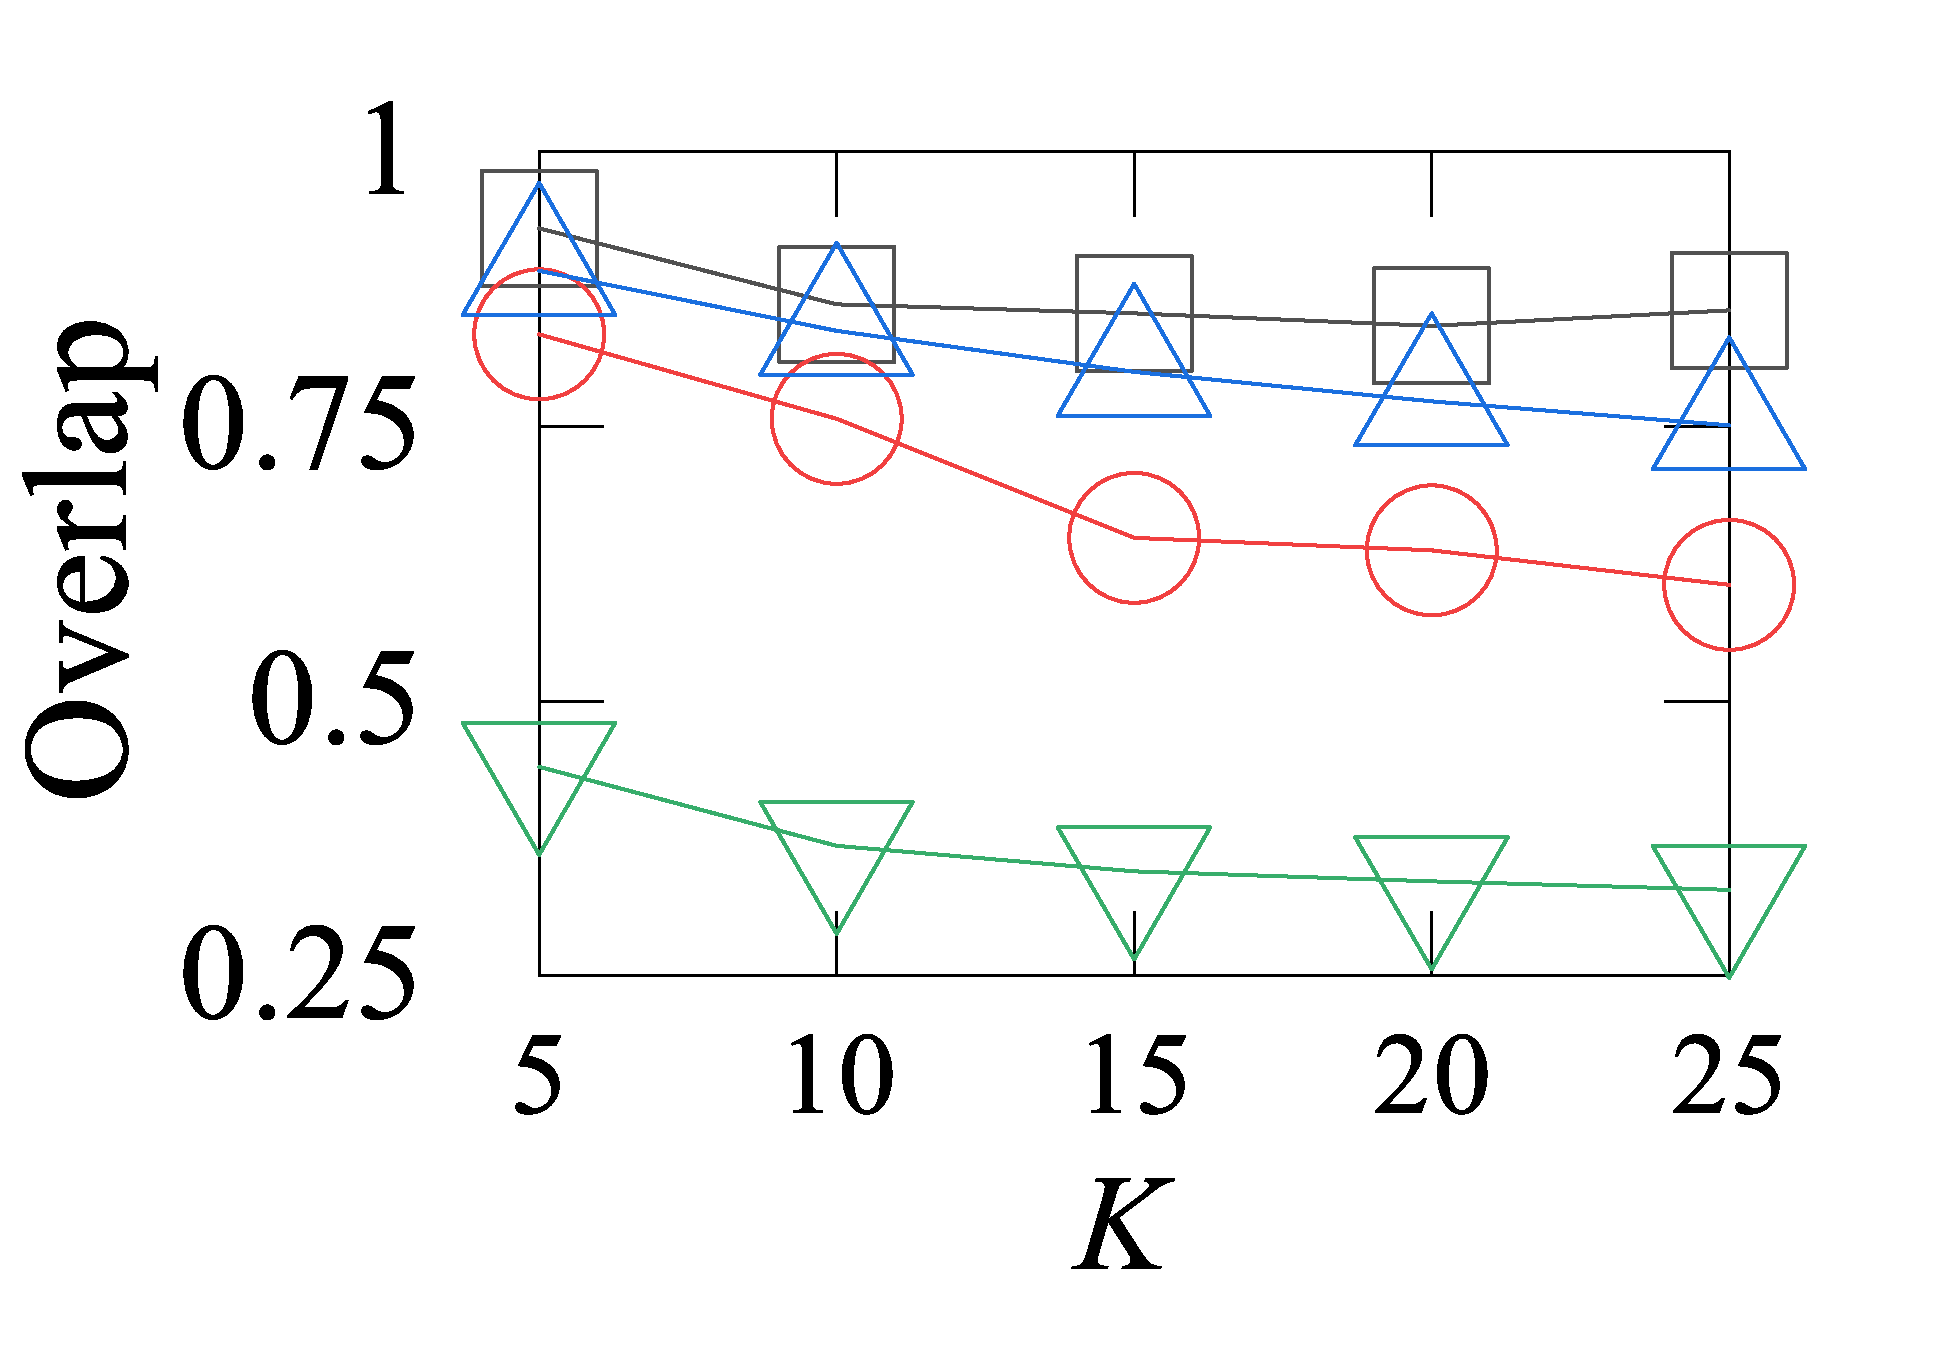
\includegraphics[width=1.7in]{figs/partition-k-medium-fr.eps}
 \label{fig:partition-k-medium-fr}
}\hspace{-3mm}
\subfigure[$\rm DBP1M_{EN-FR}$]{
 \includegraphics[width=1.7in]{figs/partition-k-large-fr.eps}
 \label{fig:partition-k-large-fr}
}\hspace{-3mm}
\subfigure[$\rm DBP1M_{EN-FR}$]{
 \includegraphics[width=1.67in]{figs/scalability-partition-en-fr-2_1.eps}
 \label{fig:scalability-p-fr}
}\\
\vspace*{-6mm}
\subfigure[$\rm IDS15K_{EN-DE}$]{
 \includegraphics[width=1.7in]{figs/partition-k-small-de.eps}
 \label{fig:partition-k-small-de}
}\hspace{-3mm}
\subfigure[$\rm IDS100K_{EN-DE}$]{
 \includegraphics[width=1.7in]{figs/partition-k-medium-de.eps}
 \label{fig:partition-k-medium-de}
}\hspace{-3mm}
\subfigure[$\rm DBP1M_{EN-DE}$]{
 \includegraphics[width=1.7in]{figs/partition-k-large-de.eps}
 \label{fig:partition-k-large-de}
}\hspace{-3mm}
\subfigure[$\rm DBP1M_{EN-DE}$]{
 \includegraphics[width=1.67in]{figs/scalability-partition-en-de-2_1.eps}
 \label{fig:scalability-p-de}
}
\vspace{-4mm}
\caption{Comparison results of different batch sampling strategies}
\vspace{-3mm}
\label{fig:partition-exp}
\end{figure*}



\begin{table}[t]\small
\caption{The result of ablation study}\label{exp:abl}
\vspace*{-4mm}
\setlength{\tabcolsep}{1mm}{
\begin{tabular}{l|ccc|ccc}
\toprule
\multicolumn{1}{c|}{\multirow{2}{*}{Methods}} & \multicolumn{3}{c|}{DBP1M$_{EN-FR}$}  & \multicolumn{3}{c}{DBP1M$_{EN-DE}$}  \\ \cline{2-7}
\multicolumn{1}{c|}{} & \multicolumn{1}{c}{H@1} & \multicolumn{1}{c}{H@10} & \multicolumn{1}{c|}{MRR} & \multicolumn{1}{c}{H@1} & \multicolumn{1}{c}{H@10} & \multicolumn{1}{c}{MRR}  \\ \hline
\ClusterEA{}                    & \textbf{28.1} & 47.4 & \textbf{0.35} & \textbf{28.8} & \textbf{48.8} &  \textbf{0.35}\\
\ClusterEA{} - \SparseCSLS{}    & 27.9 & 46.2 & 0.34 & 28.4 & 46.0 &  0.34\\
\ClusterEA{} - Global Sim       & 27.6 & \textbf{48.3} & 0.34 & 28.3 & 48.7 &  \textbf{0.35}\\
\ClusterEA{} - Sinkhorn         & 20.0 & 46.1 & 0.29 & 22.7 & 46.2 &  0.30\\
\ClusterEA{} - \KMeans{}        & 26.5 & 46.2 & 0.33 & 26.8 & 47.1 &  0.33\\
\ClusterEA{} - \MetisGCN{}      & 25.3 & 45.9 & 0.32 & 25.5 & 46.5 &  0.32\\
\ClusterEA{} - Dual-AMN         & 10.0 & 24.5 & 0.15 & 6.9  & 17.7  &  0.11\\
\bottomrule
\end{tabular}}
% \vspace*{-4mm}
\end{table}


\subsection{Ablation Study}\label{sec:ablation}
In ablatoin study, we remove 
each component of \ClusterEA{} and report \HitOne{}, \HitTen{}, and \MRR{} Table~\ref{exp:abl}.
%conduct ablation studies on both DBP1M$_{EN-FR}$ and  DBP1M$_{EN-DE}$ and report the results in Table~\ref{exp:abl}.
%from IDS and DBP1M benchmarks respectively,
%We report \HitOne{}, \HitTen{}, and $MRR$ after removing each component of \ClusterEA{}.
First, after removing the \SparseCSLS{} component, the accuracy of \ClusterEA{} drops. This verifies that the \SparseCSLS{} normalization indeed resolve the geometric problems of global similarity on large-scale EA. 
Second, after removing the global similarity, \HitOne{} of \ClusterEA{} drops while \HitTen{} raises on DBP1M$_{EN-FR}$. The fluctuation on \HitTen{} may be due to the incompleteness of global similarity normalization
that disturbs the final similarity matrix. 
Specifically, 
the local similarity is normalized into nearly permutation matrices with Sinkhorn iteration, where most values of one row are close to zero. 
When fusing local and global similarity matrices, elements that are not top-1 in the local matrix will be biased towards the value of the global matrix, which is only partially normalized.
This causes the disturbance.
However,
the incompleteness of normalization does not degrade \HitOne{}. This is because the value of one row in $\mathcal{M}_{L}$ that is correctly aligned will be normalized into a higher value, providing resistance to the global matrix disturbance. 
Third, after removing the Sinkhorn iteration,  the accuracy of \ClusterEA{} drops significantly. This verifies the importance of normalizing the similarity matrices. Finally, after removing each sampler of \Sampling{},  the accuracy of \ClusterEA{} drops on all metrics. This verifies the importance of fusing information from multi-aspects, including cross-KG information and intra-KG information.

Moreover, we observe that the \KMeans{} has less influence compared with \MetisGCN{}. This is mainly due to the following two reasons. First, \KMeans{} generally clusters entities with similar embedding vectors, where each batch still suffers from geometric problems. On the contrary,  \MetisGCN{} samples batches based on the graph neighborhood information, which is a strong constriction on the learning model. Second, we apply \MetisGCN{} in both directions. In this case, it can capture more information than \KMeans{}.
By replacing its Dual-AMN model with the GCNAlign model, the accuracy of \ClusterEA{} drops significantly on all metrics. This verifies the importance of the ability of the incorporated EA model in \ClusterEA{}.

% \vspace{-3.5mm}
\subsection{Case Study: \Sampling{} Analysis}
\label{sec:exp_minibatchgeneration}

The \Sampling{} is a vital component of \ClusterEA{}. To ensure scalability, we set the batch number $K$ such that the space cost of the normalization process does not exceed the GPU memory. We also need to guarantee that our batch sampling method can produce acceptable mini-batches under different $K$ settings.
Thus, we provide a detailed analysis on varying the batch number $K$ for different batch samplers from \Sampling{} (i.e., \MetisGCN{} and \KMeans{}). Specifically, we study how much are the mini-batches generated by one sampler acceptable as the percentage of equivalent entities that are placed into the same mini-batches (denoted as \textit{Overlap}).

Next, we report the Overlap metric and running time of the proposed sampler, where the mini-batch number $K$ of the proposed sampler is varied from 5 to 25 on IDS and is varied from 10 to 50 on DBP1M. We compare the proposed sampler with two rule-based baselines, VPS and METIS-CPS. \emph{VPS} randomly partitions seed alignments and all other entities into different mini-batches. \emph{METIS-CPS} sets the training entities with higher nodes to sample better mini-batches.
Note that both METIS-CPS and \MetisGCN{} are unidirectional. Thus, we apply these methods in both directions and report their average performance of the two directions. We report the overlap of all sampling methods on all benchmarks in Fig~\ref{fig:partition-exp}, where Figure~\ref{fig:partition-k-small-fr},~\ref{fig:partition-k-medium-fr},~\ref{fig:partition-k-large-fr},~\ref{fig:partition-k-small-de}, ~\ref{fig:partition-k-medium-de},and~\ref{fig:partition-k-large-de} are the overlap of different datasets. The results show that \KMeans{} generally outperforms two baselines on all the datasets, and its performance is stable when varying $K$. However, although better overlapped, it may result in hubness and isolation problems in mini-batches (cf. Section~\ref{sec:ablation}), thus fusing multi-aspect is essential for \ClusterEA{}. The \MetisGCN{} results in less overlapped mini-batches while still much better than the METIS-CPS. This is because METIS does not necessarily follow the guidance provided by METIS-CPS. The GNN node classification model in \MetisGCN{}, which considers the cross-entropy loss as a penalty, is forced to learn mini-batches more effectively. Since we set the training ratio to 30\%, all samplers have an overlap over 30\%, including VPS that splits mini-batches randomly.

Finally, we report the running time on DBP1M in Figure~\ref{fig:scalability-p-fr} and~\ref{fig:scalability-p-de}. Since all samplers achieve sufficiently high efficiency on IDS datasets, we do not report the running time of all samplers on IDS due to space limitations. We observe that although the result is unacceptable, VPS is the fastest sampling method. Both the proposed \MetisGCN{} and \KMeans{} are always about $2\times$ faster than the rule-based METIS-CPS when varying $K$. This is because both of them utilize machine learning models, which could be accelerated with GPU. 





